% Last modified: 2026-08-05 21:27 (Asia/Shanghai) - refine terminology and evidence alignment.
\documentclass[letterpaper,journal]{IEEEtran}

\usepackage{amsmath,amssymb,amsfonts}
\usepackage{booktabs}
\usepackage{graphicx}
\usepackage{microtype}
\usepackage{array}
\usepackage{multirow}
\usepackage{xcolor}
\usepackage{placeins}
\usepackage{dblfloatfix}
\usepackage{float}
\usepackage{cite}
\usepackage[hidelinks]{hyperref}
\usepackage{xspace}

\makeatletter
\newcommand{\includeSVG}[2][]{%
  \begingroup
  \IfFileExists{#2}{}{%
    \PackageError{RGD paper}{Missing SVG source: #2}{}}%
  \filename@parse{#2}%
  \edef\svgcompanion{\filename@area\filename@base.png}%
  \IfFileExists{\svgcompanion}{}{%
    \PackageError{RGD paper}{Missing PNG companion: \svgcompanion}{}}%
  \includegraphics[#1]{\svgcompanion}%
  \endgroup}
\makeatother

\setcounter{dbltopnumber}{2}
\renewcommand{\dbltopfraction}{0.78}
\renewcommand{\dblfloatpagefraction}{0.90}

\newcommand{\rgd}{RGD\xspace}
\newcommand{\A}{\mathcal{A}}
\newcommand{\V}{\mathcal{V}}
\newcommand{\U}{\mathcal{U}}
\newcommand{\B}{\mathcal{B}}
\newcommand{\C}{\mathcal{C}}

\definecolor{rankblue}{RGB}{190,225,250}
\definecolor{rankgreen}{RGB}{205,235,205}
\definecolor{rankyellow}{RGB}{250,235,175}
\newcommand{\rankcell}[2]{%
  \begingroup\setlength{\fboxsep}{1.2pt}%
  \colorbox{#1}{\strut\makebox[2.4em][r]{#2}}\endgroup}

\title{Recoverability-Gated Deliberation for Release-Aware Slow Reasoning in Closed-Loop Driving}

\author{Anonymous Authors}

\markboth{IEEE Transactions on Vehicular Technology}%
{Anonymous Authors: Recoverability-Gated Deliberation for Release-Aware Slow Reasoning}

\begin{document}
\maketitle
\bstctlcite{bst:etal}

\begin{abstract}
Large language models can provide deliberative reasoning for autonomous
driving, but inference latency separates the state that initiates a request
from the state in which its response becomes available. Existing asynchronous
designs preserve a fast control stream during inference, whereas deciding
whether a delayed proposal should affect the current command remains a
distinct runtime problem. This paper presents Recoverability-Gated
Deliberation~(RGD), a two-stage framework for slow-reasoner admission and
response release. At query time, RGD selects slow requests using delay
feasibility, action support, recovery-cost advantage, and scene demand. At
release, it maps the returned proposal to the observed state and admits it
only when it passes state checks, differs from the contemporaneous fast
action, and satisfies the recovery-cost condition. We also introduce
Recoverable Value of Deliberation~(R-VoD), an offline matched-rollout
diagnostic of the corrective opportunity retained at release. Experiments in
highway-env examine controlled delays, selective invocation, response traces,
and backend substitution. A zero-delay MetaDrive study examines transfer of
the common action interface. The results show that RGD preserves fast-path
continuity and allows a delayed proposal to affect the final projected command
only after it satisfies the release contract.
\end{abstract}

\begin{IEEEkeywords}
Autonomous driving, closed-loop decision making, inference latency,
large language models, recoverability, selective computation.
\end{IEEEkeywords}

\section{Introduction}
\label{sec:introduction}

\IEEEPARstart{L}{arge} language models (LLMs) and vision--language models
(VLMs) have been used for semantic scene interpretation, driving-knowledge
retrieval, and high-level decision making in autonomous driving systems
\cite{wen2023dilu,xu2024drivegpt4,shao2024lmdrive,sima2024drivelm,
 mao2023gptdriver,tvtVLNavigationCAV2025,tvtDrivingKnowledge2026,xin2026netroller}.
These capabilities supplement reactive policies with semantic context and
long-horizon intent. However, closed-loop deployment introduces a
release-time mismatch: a reasoning request is issued from one traffic
observation, while its proposal becomes available in a later state. A
high-frequency controller can maintain continuous vehicle control while a
deliberative model runs asynchronously, but the system must still decide
whether the delayed proposal should influence the current command.

Consider a closing lead vehicle and an initially open adjacent lane. The
system may request a lane-change recommendation from the slow reasoner.
During inference, traffic evolves and the fast controller continues to act.
When the response arrives, the target gap may have narrowed, the original
maneuver may no longer be admissible, or the fast controller may already
select the same or a preferable action. The release decision must therefore
test the proposal against the observed state and the contemporaneous fast
action.

Maintaining a fast control stream does not resolve this release decision. A
returned action may pass an isolated state check yet coincide with the fast
action or offer no recovery-cost advantage after traffic evolves. Both branches
therefore require a common action schema, mapper, and state-dependent
evaluator. This motivates RGD's separation of query admission from release
validation.

Recent studies address relevant parts of this process. Invocation policies use
uncertainty, scene conditions, or policy discrepancy to decide when to engage
a slow branch
\cite{hu2024fasionad,zhang2025adadrive,chen2026gvlm}. VLM-based attention
allocation prioritizes surrounding vehicles under behavioral uncertainty
\cite{tvtBehavioralAttention2026}. AsyncDriver and NetRoller preserve fast
control during model inference
\cite{chen2024asyncdriver,xin2026netroller}, while DualDrive aligns semantic
intent with a real-time policy \cite{li2026dualdrive}. Runtime-assurance
methods determine whether a candidate action may enter the actuation path
\cite{chen2022simplexdrive}. These designs primarily address invocation
timing, control continuity, or candidate safety. An explicit release-time
comparison between a delayed proposal and the contemporaneous fast action
through a shared action interface is generally not reported.

This paper addresses two questions in delayed closed-loop driving: whether the
evolved traffic state still admits a corrective action and whether the returned
proposal provides such an action at release.
Two constraints guide the design: the fast controller must remain active
throughout inference, and rejected proposals must not disrupt the control loop.
Both proposals are evaluated at the same release state through a shared action
mapper and feasibility interface.

RGD treats the slow reasoner as an optional proposal generator rather than a
replacement for the fast controller. The fast action remains the default, and
a slow proposal reaches actuation only through the shared mapper and safety
interface. This separation allows the reasoner to be changed without modifying
the release rule and makes the source of each executed action explicit.

A release state is \emph{recoverable} when the remaining maneuver window
contains at least one feasible effective alternative that remains distinct from
the fast effective action and exceeds a matched-rollout utility margin. At
query time, RGD applies online delay, support, cost, and demand conditions
before issuing a slow request. \emph{Actionability} is evaluated at release:
the returned mapped command must pass the release-state checks, differ from the
mapped fast command, and satisfy the recovery-cost margin. Recoverability
therefore describes the release state, whereas actionability describes the
returned proposal before final safety projection.

Recoverable Value of Deliberation (R-VoD) quantifies recoverability offline. It
compares alternative and fast first actions through matched rollouts from the
same logged release state under a common continuation policy. It therefore
measures the corrective opportunity remaining at release rather than the
utility of a returned slow proposal. R-VoD is a reward-defined diagnostic, not
an online value estimate, and does not enter admission or release validation.

The online gate requires scene demand, delay feasibility, action support, and
cost advantage simultaneously; high urgency alone cannot compensate for an
expired maneuver window or the absence of a supported alternative. The fast
controller supplies every action during inference. When the response arrives,
release validation evaluates the proposal in the current traffic state and
accepts it only if it passes current-state mapping, state checks, distinctness
from the fast command, and recovery-cost checks.

We evaluate RGD under a shared fast controller, slow reasoner, request budget,
and action interface across controlled delay settings. Event-level response
traces link each request to release validation and final projection. Component
analysis assesses selected admission conditions, while backend substitution and
adapter experiments examine the common action interface. Additional traffic
sweeps characterize operation under the fixed interface.

The main contributions are as follows:

\begin{enumerate}
  \item We formalize delayed deliberation through two release-time notions:
  recoverability of the current state and actionability of a returned proposal.
  We define R-VoD as an offline matched-rollout diagnostic of recoverability
  under a common continuation policy.
  \item We present RGD, which combines noncompensatory query admission with a
  release contract aligned to the fast action. The fast controller remains
  active during inference, and a delayed proposal can affect control only after
  both branches are mapped and evaluated in the observed release state through
  the shared safety interface.
  \item We conduct controlled-delay, trace-based, component,
  backend-substitution, and adapter-transfer evaluations. These studies examine
  selective invocation, release-contract enforcement, and use of the shared
  action interface under the evaluated settings.
\end{enumerate}

\section{Related Work}
\label{sec:related}

\subsection{Language-Conditioned and Generative Driving}

Language-conditioned driving methods differ in the proximity of their outputs to
vehicle actuation. At the advisory level, DiLu retrieves relevant experience
before producing an interpretable decision \cite{wen2023dilu}, and Driving with
LLMs represents traffic through object-level vectors and returns actions with
explanations \cite{chen2024drivingllms}. VLM-based systems combine visual
observations with language reasoning for navigation and motion planning
\cite{tvtVLNavigationCAV2025,tvtVLMDriver2026}, while knowledge retrieval methods
supply domain-specific context before decision making
\cite{tvtDrivingKnowledge2026}. These systems use language-conditioned
interfaces to encode scene relations and retrieve driving knowledge.

A second group places model outputs closer to the control boundary. Policy
transfer methods use language models to support vehicle decision making
\cite{titsPolicyTransfer2025}, GPT-Driver casts planning as language modeling
\cite{mao2023gptdriver}, and C-TRAIL integrates commonsense reasoning with
trajectory planning \cite{tvtCtrail2026}. Generative driving methods learn
predictive scene representations or future trajectories for downstream planning
\cite{wang2023drivedreamer,min2024driveworld,zheng2024genad,
liao2025diffusiondrive}. As outputs approach actuation, a delayed proposal may
have fewer downstream opportunities for correction and should be evaluated in
the state in which it will execute.

These studies generally focus on model capability or driving representation.
RGD instead addresses whether a delayed high-level proposal may replace the
current fast action. It operates at the interface between a slow proposal
generator and the fast controller, without introducing a new language model or
trajectory decoder. The release rule evaluates the returned proposal in the
state in which it may be executed.

\subsection{Dual Process Reasoning and Selective Computation}

Dual-process driving systems divide responsibility between a responsive policy
and a deliberative model. LeapAD uses reflection and accumulated experience,
LeapVAD adds cognitive perception, and FASIONAD coordinates both branches
through adaptive feedback \cite{mei2024leapad,ma2026leapvad,hu2024fasionad}.
DualDrive aligns semantic intent with a real-time policy, and NetRoller
connects general and specialized models through asynchronous execution
\cite{li2026dualdrive,xin2026netroller}. In each design, the fast branch
supplies immediate control while the slow branch contributes information or
actions at selected intervals.

Selective computation methods determine when the slow branch should run.
AdaDrive and AdaThinkDrive adapt deliberation depth to scene demand
\cite{zhang2025adadrive,luo2025adathinkdrive}, and G-VLM calibrates invocation
from the discrepancy between lightweight and multimodal policies
\cite{chen2026gvlm}. Behavioral Attention uses a VLM to allocate attention
among surrounding vehicles under behavioral uncertainty
\cite{tvtBehavioralAttention2026}. These invocation signals are evaluated before
inference begins, when neither the returned action nor the release state is
known. RGD supplements invocation selection with release-time evaluation against
the contemporaneous fast action.

Query-time selection and release-time validation serve different purposes. The
first determines whether slow computation should begin; the second determines
whether its output remains useful after the state has changed. RGD retains both
decisions explicitly rather than treating a successful request as sufficient
for release.

Metareasoning balances expected decision improvement against computational cost.
Time-bounded and anytime methods schedule reasoning under a finite budget
\cite{russell1991metareasoning,boddy1994deliberation,zilberstein1996anytime,
cserna2017planning}, and concurrent planning permits an executor to continue
acting while a planner computes \cite{elboher2023concurrent}. In driving, an
estimate made at query time can differ from the opportunity available at
release because traffic evolves while the fast controller continues to act.
R-VoD operationalizes the remaining corrective opportunity through matched
rollouts.

\subsection{Runtime Safety, Delay, and Viability}

Timing mechanisms preserve control during inference. AsyncDriver separates
language-model planning from real-time control
\cite{chen2024asyncdriver}, NetRoller keeps a specialized driving model active
\cite{xin2026netroller}, and event-triggered or adaptive-computing strategies
regulate update frequency \cite{tabuada2007event,li2021edgecomputing}.
Delay-aware control further models state evolution during input lag
\cite{molnar2023delay}. At the assurance layer, Simplex-based systems revert to
a trusted controller when a learned action fails an acceptance test
\cite{chen2022simplexdrive}, and formal viability methods characterize
admissible motion under dynamic constraints
\cite{shalevshwartz2017rss,liniger2019viability}.

These approaches address timing, invocation, or candidate safety. They do not
generally formulate a comparison between a delayed proposal and the
contemporaneous fast action as a separate release-time decision. RGD complements
rather than replaces runtime safety mechanisms. The shared safety interface
checks whether a mapped action can enter actuation, while release validation
additionally tests whether the delayed proposal is distinct from, and has a
recovery-cost advantage over, the contemporaneous fast action. A safe but
equivalent proposal therefore leaves the fast action unchanged. The final safety
shield remains active after selection.

\section{Recoverability-Gated Deliberation}
\label{sec:method}

RGD separates a slow-reasoner call into query admission and release validation.
Admission determines whether the scene warrants deliberation and whether a
feasible alternative is supported under the expected delay. Release validation
checks the returned proposal in the observed release state. The fast controller
supplies the executed action while inference is pending and whenever either
stage rejects the slow path.

A release state $s_r$ is \emph{recoverable} if it contains a feasible effective
alternative that remains distinct from the fast effective action and exceeds
its matched-rollout utility by at least $\epsilon$. R-VoD measures this
state-level opportunity offline. A returned proposal is \emph{actionable at
release} only if its mapped command passes the contemporaneous state checks,
differs from the mapped fast command, and satisfies the proposal-specific
recovery-cost margin. The final safety projection may still map an authorized
command to the fast executed action. Thus, R-VoD and release validation serve
complementary rather than interchangeable roles.

\begin{figure*}[!t]
  \centering
  \includeSVG[width=\textwidth]{figures/sturcture_new.svg}
  \caption{RGD architecture and information flow. Query admission requires
  delay feasibility ($L_t$), action support ($A_t$), cost advantage ($H_t$),
  scene demand ($N_t$), and resource availability. At release, a returned
  proposal is evaluated through current-state mapping, recomputed state checks,
  mapped-command distinctness from the fast branch, and a proposal-specific cost
  margin before the shared safety projection. The optional driving-memory block
  was disabled in the frozen evaluations. Matched first-action rollouts from release
  snapshots provide offline R-VoD labels.}
  \label{fig:overview}
\end{figure*}

As shown in Fig.~\ref{fig:overview}, the online path contains the two gates,
whereas the offline branch constructs R-VoD labels from matched first-action
rollouts. The fast controller remains active at every cycle. Driving memory can
provide context after admission, but it does not alter either gate and is not
used in the reported frozen runs.

The architecture imposes a non-interference contract on slow reasoning. A slow
request never suspends the fast controller, and a missing response, mapping
failure, or rejected release leaves the fast command selected. The reasoner is
therefore a proposal source rather than a second controller. This boundary
prevents inference latency and response-format errors from changing the control
cadence.

The release comparison is action-aligned. Both fast and slow proposals first
enter the same mapped command space, after which the same feasibility and cost
interfaces are applied. Semantically equivalent language outputs are therefore
treated as the same maneuver, and backend-specific wording cannot create an
artificial action difference. The shared final safety shield remains the last
stage for either source.

\subsection{Query and Release Process}

At frame $t$, the ego vehicle observes state $s_t$. The fast policy $\pi_f$ is
mapped by the shared action mapper to $a_t^f$. Both branches use this mapper and
the same final safety projection $\Phi(s,a)$, which projects a mapped command
to its final executable action in state $s$. The mapper converts each proposal
into a command and target speed; different expressions are equivalent when they
induce the same mapped behavior. The high-level action domain comprises
lane-left, lane-hold, lane-right, accelerate, and decelerate, all mapped through
the same simulator interface.

The returned proposal is mapped in the observed release state $s_r$. A
lane-change or speed command available at query time may no longer be valid;
a mapping or feasibility failure leaves $a_r^f$ selected.

The delay estimate is used only for admission. The actual release frame $r$ is
the first control frame at which the response is available, and returned and
fast actions are evaluated in the observed state $s_r$. Responses unavailable
before episode termination are not released.

\subsection{Offline Measure of Corrective Opportunity}

Offline matched rollouts quantify the corrective opportunity at release. At
each logged release snapshot $s$, let $a_{\mathrm{eff}}^f=\Phi(s,a^f)$ denote the effective
fast first action after the shared mapper and final safety projection.
$\mathcal D(s)$ contains feasible effective first actions that remain distinct
from $a_{\mathrm{eff}}^f$ after the same stages, and
$\mathcal C(s)=\{a_{\mathrm{eff}}^f\}\cup\mathcal D(s)$. The matched-rollout
utility and Recoverable Value of Deliberation (R-VoD) are
\begin{equation}
\begin{aligned}
J(s,a)&=
\frac{\sum_{k=0}^{K-1}\gamma^k\bar r_k(s,a)}
     {\sum_{k=0}^{K-1}\gamma^k}
-\lambda_{\mathrm{col}}\mathbb{I}_{\mathrm{col}}(s,a),\\
\mathrm{R\text{-}VoD}(s)&=
\max_{a\in\mathcal C(s)}
\bigl[J(s,a)-J(s,a_{\mathrm{eff}}^f)\bigr].
\end{aligned}
\label{eq:rvod}
\end{equation}
Here, $K$ is the common positive rollout horizon, $\gamma\in(0,1]$ is the
discount factor, $\bar r_k$ is the normalized simulator reward, and
$\lambda_{\mathrm{col}}>0$ weights the collision indicator
$\mathbb{I}_{\mathrm{col}}(s,a)$. Reward increments after termination are set
to zero. Only the first effective action is changed; the fast policy supplies
the continuation.
Because $a_{\mathrm{eff}}^f\in\mathcal C(s)$, R-VoD is nonnegative and equals
zero when no alternative improves the matched fast continuation. A state is
labeled corrective when $\mathrm{R\text{-}VoD}(s)\geq\epsilon$, where
$\epsilon>0$ is a fixed diagnostic margin.

The matched design fixes the logged release state, traffic realization,
maximum horizon, continuation policy, and termination rule. Accordingly,
$J(s,a)$ is an offline, reward-defined utility for the diagnostic; it is not
queried by the online gate. By contrast, $c_t(a)$ is a runtime recovery-cost
score used to rank current actions at admission and to test a returned command
at release. The two quantities are purpose-built for different decisions and
are not interchangeable.

Changing only the first effective action isolates the corrective opportunity
available in the release state under the common simulator continuation. R-VoD
therefore does not reward response length, explanation quality, or a particular
LLM backend. It supplies a state-level label against which an admission policy
can be evaluated. Release validation tests whether a returned proposal satisfies
the online release contract; the final projection separately determines its
executed effect.

\subsection{Query Admission}

The online gate evaluates four conjunctive conditions. All must hold; high
scene demand cannot compensate for an expired maneuver window.

Let $\mathcal A_t$ denote the current mapped action set. The fixed evaluator
assigns each member a normalized recovery cost
$c_t:\mathcal A_t\rightarrow[0,1]$, where lower values are preferred, and a
normalized support $u_t(a)\in[0,1]$. Let $\mathcal D_t^{\mathrm{alt}}$ contain
feasible actions whose mapped commands differ from $a_t^f$. For each
alternative action family $m$, its support $\bar u_{t,m}$ is the largest
$u_t(a)$ among feasible members; an unavailable family contributes zero.
\textit{Action support} $A_t$ is the mean of these family-wise maxima and is
set to zero when no alternative family is available or the evidence is
incomplete. Let
$c_t^{\mathrm{alt}}=\min_{a\in\mathcal D_t^{\mathrm{alt}}}c_t(a)$ when the set is
nonempty and $c_t^{\mathrm{alt}}=c_t(a_t^f)$ otherwise.

The remaining gate factors are
\begin{equation}
\begin{aligned}
L_t&=\operatorname{clip}\!\left(
1-\frac{\widehat\ell_t+\rho_t}{\max(d_t,\varepsilon_d)},0,1\right),\\
H_t&=\operatorname{clip}\!\left(
\frac{[c_t(a_t^f)-c_t^{\mathrm{alt}}]_+}{\kappa},0,1\right),\\
N_t&=\max\{n_t^{\mathrm{haz}},n_t^{\mathrm{int}}\}.
\end{aligned}
\label{eq:gate_factors}
\end{equation}
Here, $L_t$ is delay feasibility, $H_t$ is cost advantage, and $N_t$ is scene
demand. The terms $n_t^{\mathrm{haz}},n_t^{\mathrm{int}}\in[0,1]$ are normalized
hazard and interaction evidence, respectively. The timing quantities
$d_t$, $\widehat\ell_t$, $\rho_t\geq0$, and $\varepsilon_d>0$ use the same time
unit; $d_t$ is the estimated time to the earliest active maneuver constraint,
$\rho_t$ is a timing reserve, and $\varepsilon_d$ is a timing regularizer.
The positive constant $\kappa$ normalizes the recovery-cost advantage. A bounded
planning horizon replaces $d_t$ when no finite constraint is active. The
operator $[x]_+=\max\{x,0\}$, and
$\operatorname{clip}(x,0,1)=\min\{1,\max\{0,x\}\}$. If
$\mathcal D_t^{\mathrm{alt}}$ is empty, $H_t=0$. The maximum in $N_t$ avoids
counting correlated hazard and interaction evidence twice.

The factors encode different necessary conditions. $L_t$ tests whether
computation fits within the maneuver window, $A_t$ requires support across
alternative action families, $H_t$ requires at least one lower-cost
alternative, and $N_t$ establishes a reason to deliberate. Their conjunction is
deliberately noncompensatory: high scene demand cannot offset expired timing,
and broad action support cannot offset the absence of a cost advantage. This
structure preserves the operational meaning of each gate factor across delay
settings.

Resource availability, including the request budget, cooldown, and executor
status, is represented by $v_t\in\{0,1\}$; $v_t=1$ also requires that no slow
request is pending. The admission rule is
\begin{equation}
\begin{aligned}
q_t=\mathbb{I}\big[&v_t=1\wedge L_t\geq\tau_L\wedge A_t\geq\tau_A\\
&\wedge H_t\geq\tau_H\wedge N_t\geq\tau_N\big],
\end{aligned}
\label{eq:query_admission}
\end{equation}
where $\mathbb{I}[\cdot]$ is the indicator function and
$\tau_j\in(0,1]$, $j\in\{L,A,H,N\}$, are generic gate floors selected on
development scenarios and fixed before evaluation.

If latency evidence, the action-cost vector, or the slow executor is
unavailable, the corresponding condition is false and the fast controller
continues without issuing a slow request.

\subsection{Release Validation}

At the actual release frame $r$, let $y_r$ be the returned response and
$\mathcal M$ the shared current-state mapper. The fast policy produces the
mapped fast command $a_r^f$ from the same state. If $\mathcal M(s_r,y_r)$ is
undefined, the release gate is set to zero and the fast command is retained.
Otherwise, let $\widetilde a_r^{\mathrm{sl}}=\mathcal M(s_r,y_r)$ denote the
mapped slow command. Only $A_r$, $H_r$, and $N_r$ are recomputed from $s_r$;
$L_t$ is used only for query admission. Let $\mathcal V_r\subseteq\mathcal A_r$
denote the feasible mapped commands when these release-state conditions hold,
and let $\mathcal V_r=\varnothing$ otherwise. If a condition fails or
$\widetilde a_r^{\mathrm{sl}}\notin\mathcal V_r$, the fast command is retained.
Conditional on these checks, the remaining test in Fig.~\ref{fig:overview} is
\begin{equation}
\begin{aligned}
g_r=\mathbb{I}\big[&\widetilde a_r^{\mathrm{sl}}\neq a_r^f\\
&\wedge c_r(a_r^f)-c_r(\widetilde a_r^{\mathrm{sl}})\geq\tau_R\big].
\end{aligned}
\label{eq:release_stages}
\end{equation}
Here, $\tau_R\in(0,1]$ is a generic release margin under
$c_r(\cdot)\in[0,1]$ and is fixed before evaluation.

The mapped slow command is selected when $g_r=1$; otherwise, the fast command is
retained. The shared safety projection $\Phi$ then produces the executed action.
Distinctness is tested between mapped commands before $\Phi$, so the shield may
still map an authorized slow command to the same executed command as the
projected fast action. Post-projection distinctness is therefore an execution
outcome reported separately. The release-state $H$ condition establishes that a
lower-cost alternative exists, while the final term in
\eqref{eq:release_stages} tests whether the returned mapped command meets the
required margin. No R-VoD label enters this online decision.

Release validation is stricter than a slow-action safety test. Feasibility asks
whether the mapped proposal can execute in $s_r$, distinctness asks whether it
differs from the contemporaneous mapped fast command, and the final comparison
asks whether it satisfies the recovery-cost margin. A proposal admitted at
query time receives no persistent authority; all response-specific checks use
the observed release state.

\FloatBarrier
\section{Experiments and Discussion}
\label{sec:experiments}

\subsection{Experimental Setup}

We evaluate RGD on the highway-env \cite{lesort2018highwayenv} and MetaDrive
\cite{li2023metadrive} closed-loop simulators with Qwen3-8B
\cite{qwen3technicalreport} as the default slow reasoner. The main highway-env
experiments operate at 10~Hz for 30~s. Each comparison shares a fixed seed
cohort, action schema, fast controller, and evaluation rule; gate development,
main evaluation, and mechanism analysis use separate cohorts. The main analyses
use 30 seeds; the component analysis uses a separate 20-seed cohort. Unless
stated otherwise, intervals denote 95\% percentile bootstrap confidence
intervals with simulator seed as the resampling unit. R-VoD is computed only
after release through matched first-action rollouts. Gate floors, normalization
constants, and corrective margins are selected on the development cohort and
remain fixed throughout the reported evaluation.

The experiment suite gives each analysis a distinct evidentiary role.
System-level context places the closed-loop implementation in established task
settings. The delay sweep tests whether admission allocates slow computation
according to the available maneuver window, while the response trace tests the
release contract after the traffic state evolves. The component study examines
how selected admission conditions shape the states sent to the slow path.
Backend substitution evaluates the common action interface under different
reasoners, and the traffic and simulator studies characterize the fixed
interface across evaluated road structures and adapters. This organization
links each result to a specific system property.

\begin{table*}[!t]
\centering
\caption{Protocol-context values in the PADriver setting (not a head-to-head comparison).}
\label{tab:padriver}
\footnotesize
\renewcommand{\arraystretch}{1.02}
\setlength{\tabcolsep}{3.8pt}
\begin{tabular*}{0.92\textwidth}{@{\extracolsep{\fill}}lrrrrrr@{}}
\toprule
\textbf{Method} & \textbf{Distance (m)} & \textbf{Speed (km/h)} &
\textbf{Saf.} & \textbf{Kep.} & \textbf{Completed} &
\textbf{Runtime (s/frame)}\\
\midrule
Driving with LLMs & 411 & 49.42 & 0.49 & 0.56 & 20 & 48.0\\
GPT-Driver & 428 & 51.40 & 0.45 & 0.52 & 23 & 36.2\\
DiLu & 386 & 46.29 & 0.60 & 0.72 & 28 & 24.1\\
PADriver--Normal & 603 & 72.47 & 0.91 &
0.92 & 25 & 1.4\\
RGD (ours) & 611 & 73.60 & 0.75 & 0.86 &
29 & 0.0376\\
\bottomrule
\end{tabular*}
\end{table*}

\subsection{System-Level Context}

Following the PADriver experimental conditions \cite{kou2025padriver}, we
evaluate RGD and report the resulting values alongside source-reported
context. The source entries retain their original definitions and evaluation
scope; Table~\ref{tab:padriver} is therefore not a statistical head-to-head
comparison. Within this protocol context, RGD completes 29 of 30 runs, records
611~m and 73.60~km/h, and operates at 37.6~ms per frame without a dedicated
training phase on the evaluation environment. The fast controller remains
active at every frame, whereas the slow reasoner is invoked selectively. Saf.
and Kep. denote safe-distance keeping and lane keeping, respectively.

Hu et al.~\cite{tvtVLNavigationCAV2025} define success as 30 consecutive
collision-free frames. We adopt their three density settings and ten seeds per
setting with no added delay. Fig.~\ref{fig:hu_protocol} reports success rates
alongside published values, and Table~\ref{tab:hu_protocol} provides RGD's
operating metrics under the settings stated in the source paper.

\begin{figure}[!ht]
  \centering
  \includegraphics[width=\columnwidth]{figures/fig2_hu2025_protocol_comparison.pdf}
  \caption{Success-rate context in the highway-env settings of Hu et al.
  GPT-4, GRAD, and DeepSeek-R1 are source-reported values; their placement with
  RGD is not a head-to-head statistical comparison.}
  \label{fig:hu_protocol}
\end{figure}

\begin{table}[!ht]
\centering
\caption{RGD operating metrics under the source protocol context of Hu et al.}
\label{tab:hu_protocol}
\scriptsize
\renewcommand{\arraystretch}{1.04}
\setlength{\tabcolsep}{2.3pt}
\begin{tabular*}{\columnwidth}{@{\extracolsep{\fill}}lrrrr@{}}
\toprule
\textbf{Setting} & \textbf{Dist. (m)} & \textbf{Speed (m/s)} &
\textbf{Requests/ep.} & \textbf{Runtime (ms/frame)}\\
\midrule
4L / 2.0 & 69.29 & 23.84 & 1.0 & 58.9\\
4L / 2.5 & 66.19 & 22.76 & 1.0 & 65.2\\
5L / 3.0 & 52.38 & 17.38 & 0.8 & 50.1\\
\bottomrule
\end{tabular*}
\end{table}

Under the settings stated by Hu et al., RGD attains 100\% success at 4L/2.0
and 4L/2.5. At 5L/3.0, it attains 80\% success and schedules 0.8 slow-path
requests per episode. Table~\ref{tab:hu_protocol} uses safety-qualified speed,
assigns zero to unsuccessful episodes, and averages requests over the ten
episodes in each setting. The per-frame runtime remains below 66~ms in all
three settings.

\subsection{Delay-Controlled Allocation and Component Evidence}

\subsubsection{Zero Added Delay Reference}

The zero-delay experiment provides a reference in which all six allocation
policies share the same fast controller, slow reasoner, request budget, and
feasibility interface; only the request and release rules differ. The
subsequent delay sweep uses the same seeds to examine how delay feasibility
changes slow-path allocation.

\begin{figure*}[!t]
  \centering
  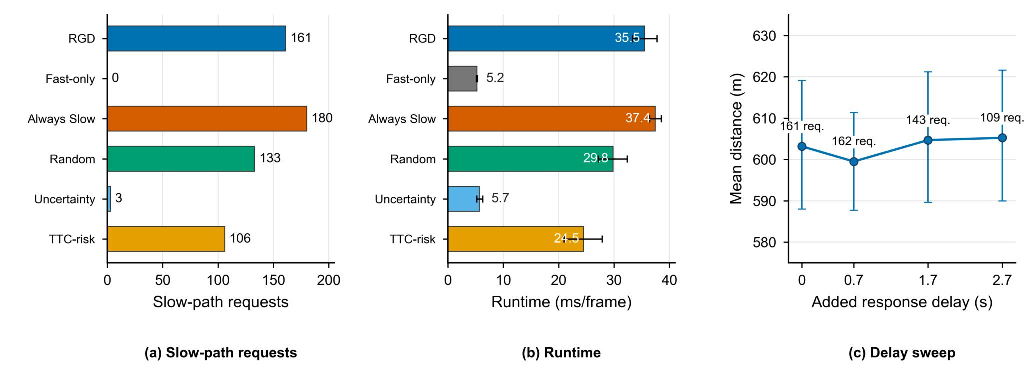
\includegraphics[width=0.88\textwidth]{figures/fig_zero_delay_latency_extension.pdf}
\caption{Zero-delay policy comparison and RGD delay sweep: (a) slow-path
request totals, (b) per-frame runtime, and (c) distance and requests versus
added delay. Request counts aggregate 30 seeds; error bars denote 95\%
seed-bootstrap confidence intervals for runtime and distance.}
  \label{fig:zero_delay_extension}
\end{figure*}

Without added delay, Fig.~\ref{fig:zero_delay_extension}(a)--(b) shows that RGD
schedules fewer slow-path requests and has a lower per-frame runtime than Always
Slow. This result shows that query admission reduces continual slow-path use
under the same fast controller and slow reasoner.

Across the delay sweep in Fig.~\ref{fig:zero_delay_extension}(c), distance
remains within overlapping confidence intervals while the request count
decreases at longer added delays. This allocation pattern is consistent with
the delay-feasibility condition becoming more selective as the response interval
grows. The fixed gate therefore adjusts its invocation rate without per-delay
retuning.

\subsubsection{Allocation With a 1.7-s Added Delay}

The 1.7-s experiment examines how RGD processes a slow response after the
traffic state has evolved. The fast controller, slow reasoner, request budget,
seed cohort, and feasibility interface remain fixed. Fig.~\ref{fig:operating_profile}
reports the response-validation stages and the resulting release decisions.

\begin{figure*}[t]
  \centering
  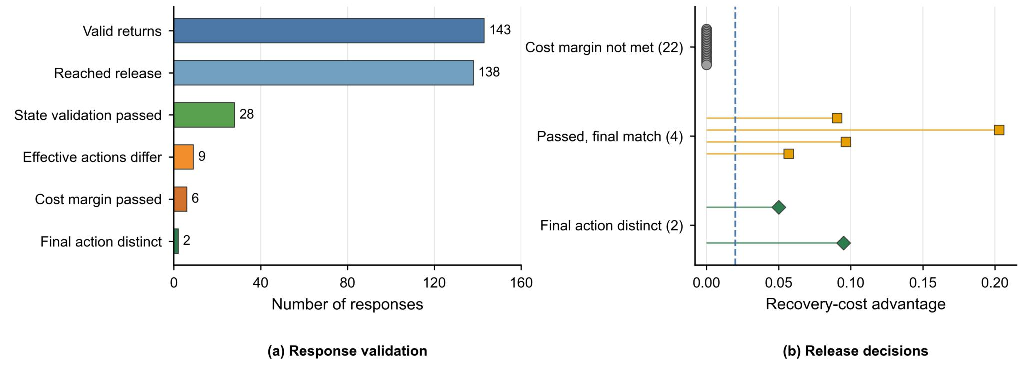
\includegraphics[width=0.88\textwidth]{figures/fig2_v13_main_evidence.pdf}
\caption{Response-validation funnel at a 1.7-s added delay: (a) returned,
release-reached, state-valid, mapped-distinct, cost-qualified, and
projection-distinct responses; (b) recovery-cost advantages and final outcomes
for the 28 state-valid responses. Stage counts aggregate the 30-seed main
cohort; the dashed line denotes the release margin $\tau_R$.}
\label{fig:operating_profile}
\end{figure*}

\begin{figure*}[t]
  \centering
  \includegraphics[width=0.88\textwidth]{figures/fig3_v13_component_analysis.pdf}
\caption{Admission-component analysis: (a) slow-path request totals, (b)
additional release states selected by the $L$, $A$, or $H$ ablation, and (c)
R-VoD-labeled corrective-state-rate differences computed as Full RGD minus the
corresponding ablation. Counts aggregate the separate 20-seed mechanism cohort;
error bars denote 95\% confidence intervals.}
  \label{fig:components}
\end{figure*}

Table~\ref{tab:multi_llm} reports a separate 30-seed backend evaluation under
the 1.7-s setting. ``Calls'' denotes successful service responses rather than
request attempts in the main cohort.

\begin{table}[!t]
\centering
\caption{Backend substitution under a fixed RGD interface at a 1.7-s added delay.}
\label{tab:multi_llm}
\footnotesize
\renewcommand{\arraystretch}{1.04}
\setlength{\tabcolsep}{3.0pt}
\begin{tabular*}{\columnwidth}{@{\extracolsep{\fill}}lrrr@{}}
\toprule
\textbf{Reasoner} & \textbf{Calls} & \textbf{Distance (m)} & \textbf{Completion}\\
\midrule
Qwen3-8B & 138 & 599.16 & 0.97\\
Qwen3.5-4B & 138 & 599.16 & 0.97\\
Qwen2.5-7B & 122 & 599.12 & 0.97\\
GPT-5.6-sol & 112 & 603.39 & 0.97\\
GPT-5.6-terra & 132 & 599.16 & 0.97\\
GPT-5.6-luna & 133 & 599.16 & 0.97\\
Fable-5 & 137 & 599.16 & 0.97\\
\bottomrule
\end{tabular*}
\end{table}

The fixed delay ensures that each returned proposal is evaluated in a state
later than the state that initiated the request. RGD therefore applies a
returned proposal only after all release checks.

\subsubsection{Response Validation and Component Effects}

Response traces follow each request from admission through response validation,
current-state mapping, and actuation. At the same 1.7-s added delay, the
leave-one-out variants use a separate 20-seed cohort; each removes one admission
condition while retaining the release procedure.

Under the 1.7-s delay, 143 RGD requests return valid responses and 138 reach
release before episode termination. Current-state checks admit 28 responses to
the release comparison; nine mapped slow commands differ from the contemporaneous
fast command, and six satisfy the recovery-cost margin. After the shared final
projection $\Phi$, four of these authorized commands match the projected fast
command and two remain distinct. Fig.~\ref{fig:operating_profile}(a) reports
the complete event funnel, while panel~(b) summarizes all 28 state-valid
outcomes. Thus, a delayed proposal can affect the final command only after it
satisfies the release contract and remains distinct after projection; otherwise,
the fast action remains in control.

Fig.~\ref{fig:components}(a)--(b) shows that removing $L$, $A$, or $H$ changes
both the number of requests and the release states selected by the gate.
Panel~(c) reports the R-VoD-labeled corrective-state-rate difference between
Full RGD and each ablation with 95\% seed-bootstrap confidence intervals. The
$H$ contrast has a confidence interval entirely above zero, directly linking
the online cost-advantage condition to the corrective-state composition of the
selected cohort. The selection changes in panels~(a)--(b) further show that
$L$ and $A$ shape which states are sent to the slow path. Together, these
analyses establish the complementary roles of delay feasibility, action support,
and recovery-cost advantage in the admission rule.

The corrective-state rate in Fig.~\ref{fig:components}(c) is labeled offline by
R-VoD, whereas $H_t$ is computed online from the recovery-cost evaluator
$c_t$. The two quantities serve different roles: $H_t$ ranks current candidate
actions before a request is issued, whereas R-VoD labels the opportunity that
remains at the observed release state through matched rollouts. The $H$
contrast therefore connects an online admission signal with a separately
constructed release-state diagnostic.

\subsection{Reasoner-Interface Evaluation}

We replace only the slow reasoner while retaining the RGD gate, action schema,
and fallback path. Table~\ref{tab:multi_llm} reports closely aligned distance
and completion values across the seven evaluated backends, from local models to
API services. Successful service responses range from 112 to 138, whereas mean
distance ranges from 599 to 603~m and every backend attains a completion rate
of 0.97. All backends use the same action mapping, current-state validation,
and recovery-cost comparison. Under this shared interface, the observed
system-level point estimates remain closely aligned across the evaluated
backends.

% Keep Tables VI--VIII in one ordered full width float so IEEEtran cannot defer
% the comparison tables beyond Section IV while waiting for a single column float.
\begin{table*}[!t]
\centering
\begin{minipage}[t]{0.47\textwidth}
\centering
\caption{RGD outcomes under lane and density settings.}
\label{tab:traffic_stress}
\scriptsize
\renewcommand{\arraystretch}{1.05}
\setlength{\tabcolsep}{2.0pt}
\begin{tabular*}{\linewidth}{@{\extracolsep{\fill}}lrr@{}}
\toprule
\textbf{Lanes/Density} & \textbf{Distance (m)} &
\textbf{Successful runs (/30)}\\
\midrule
4L/2.0 & 599 & 29\\
4L/3.0 & 478 & 23\\
5L/2.0 & 629 & 30\\
5L/3.0 & 429 & 20\\
6L/2.0 & 611 & 28\\
6L/3.0 & 453 & 20\\
\bottomrule
\end{tabular*}
\end{minipage}%
\hfill
\begin{minipage}[t]{0.47\textwidth}
\centering
\caption{Compound-hazard task context in MetaDrive (source-context comparison).}
\label{tab:policy_transfer}
\scriptsize
\renewcommand{\arraystretch}{1.06}
\setlength{\tabcolsep}{1.8pt}
\begin{tabular*}{\linewidth}{@{\extracolsep{\fill}}llrr@{}}
\toprule
\textbf{Method} & \textbf{Scene} & \textbf{Safety (\%)} & \textbf{Speed (m/s)}\\
\midrule
\multirow{3}{*}{ASR-RL~\cite{titsPolicyTransfer2025}}
& A & 99.2 & 7.1\\
& B & 98.3 & 8.6\\
& C & 97.9 & 6.8\\
\midrule
\multirow{3}{*}{RGD (ours)}
& A & 100.0 & 4.8\\
& B & 94.8 & 7.0\\
& C & 84.6 & 6.9\\
\bottomrule
\end{tabular*}
\end{minipage}
\vspace{5pt}

\centering
\caption{Maneuver and traffic-density task context (source-context comparison).}
\label{tab:bua_transfer}
\footnotesize
\renewcommand{\arraystretch}{1.06}
\setlength{\tabcolsep}{4.0pt}
\begin{tabular*}{0.94\textwidth}{@{\extracolsep{\fill}}l*{8}{r}@{}}
\toprule
& \multicolumn{5}{c}{\textbf{Traffic Scenario}}
& \multicolumn{3}{c}{\textbf{Left Turn Traffic Density}}\\
\cmidrule(lr){2-6}\cmidrule(lr){7-9}
\textbf{Method} & \textbf{Left} & \textbf{Right} & \textbf{Straight} &
\textbf{Merge} & \textbf{Round.} & \textbf{1.0} & \textbf{2.0} &
\textbf{3.0}\\
\midrule
VLM attention allocation \cite{tvtBehavioralAttention2026} &
0.966 & 0.991 & 0.984 & 0.987 & 0.974 & 0.975 & 0.961 & 0.948\\
RGD (ours) & 0.842 & 0.908 & 0.868 & 0.986 & 0.747 & 0.906 & 0.763 & 0.601\\
\bottomrule
\end{tabular*}
\end{table*}

\subsection{Evaluation Across Traffic and Simulators}

\subsubsection{Traffic Structure}
\label{subsec:traffic}

The auxiliary sweep includes the default 4L/2.0 setting and five lane/density
variants without retuning the gate. Table~\ref{tab:traffic_stress} reports mean
distance and successful runs over 30 episodes per setting. At density 2.0,
successful runs range from 28 to 30 and mean distance from 599 to 629~m.
Across all six cells, the fixed configuration completes 20--30 runs. These
results describe operation of the same interface under the evaluated traffic
structures.

\subsubsection{Simulator Transfer}

The MetaDrive experiment introduces simulator-specific observation and action
adapters at zero response delay, with no modification to the gate configuration
used in highway-env. The shared action schema, admission rule, and fallback
order are applied without retuning. This study evaluates transfer of the common
action interface across heterogeneous simulator dynamics; delayed release-time
behavior is characterized by the highway-env experiments.

Fig.~\ref{fig:simulator_scenes} visualizes representative frozen
cross-simulator traces. The upper row contains highway-env highway, merge,
roundabout, and intersection states; the lower row contains the corresponding
MetaDrive state reconstructions. The paired layouts expose the same discrete
high-level action schema in straight-road, merging, circulating, and
cross-traffic geometries. The scenes provide visual context for the quantitative
transfer studies.

Road geometry, traffic representation, and simulator dynamics differ across
the two rows, yet each panel uses the same mapper, admission rule, and fast-path
fallback. The zero-delay MetaDrive study exercises the common release interface
through the simulator adapter. The MetaDrive panels reconstruct the logged ego
state and recorded task-relevant neighbors at the selected frame, providing a
direct view of the adapter boundary while preserving the traffic configuration
used by the frozen evaluation.

\begin{figure*}[!t]
  \centering
  \includeSVG[width=\textwidth]{figures/fig_simulator_scenes.svg}
  \caption{Representative frozen closed-loop states under the shared RGD
  interface. The upper row shows highway-env: (a) highway, (b) merge,
  (c) roundabout, and (d) intersection. The lower row shows recorded-state
  reconstructions of the corresponding MetaDrive scenes: (e) highway,
  (f) merge, (g) roundabout, and (h) intersection. The ego vehicle is shown in
  green in every panel.}
  \label{fig:simulator_scenes}
\end{figure*}

\subsection{Evaluation on Additional Scenario Families}

The published ASR-RL and VLM-attention rows retain their source definitions and
evaluation scopes, whereas the RGD rows are measured in this work. The values
provide task-level context rather than a common-protocol statistical ranking.

\subsubsection{Compound Hazard Scenes}

Following the experimental conditions stated by ASR-RL
\cite{titsPolicyTransfer2025}, the MetaDrive evaluation covers pedestrian
crossing (A), uncontrolled intersection (B), and combined vehicle-pedestrian
traffic (C), each with 1,000 episodes. Table~\ref{tab:policy_transfer} reports
the RGD results alongside source-reported ASR-RL context. RGD attains 100\%
collision-free safety in Scene~A and applies the same gate configuration across
the three compound-hazard scenes without policy-library training or
scenario-specific retuning.

\subsubsection{Maneuver and Density Changes}

Following the settings stated in the source paper, five maneuver classes and a
left-turn density sweep are evaluated at 2~Hz for 30~s with 1,000 episodes per
cell. Table~\ref{tab:bua_transfer} reports the RGD success rates alongside
published VLM attention-allocation values
\cite{tvtBehavioralAttention2026} as task-level context. RGD achieves 0.986 on
merge, and the same high-level action interface and gate logic are applied
across highway, junction, and curved-road maneuver families.

\subsection{Discussion}

RGD separates three related decisions. Before computation, admission asks
whether a supported lower-cost alternative can remain useful within the expected
response interval. After state evolution, release validation asks whether the
returned proposal satisfies the contemporaneous contract relative to the action
the fast controller would now take. The final safety projection then determines
the executed command. This organization distinguishes recoverability of the
release state, authorization of the returned proposal, and post-projection
execution outcomes.

The controlled-delay studies characterize the admission decision, and the
response trace evaluates the release contract. The delay sweep shows that the
fixed admission rule changes slow-path allocation as the response interval
changes. The trace follows each proposal through current-state mapping,
recomputed state checks, mapped-command distinctness, recovery-cost comparison,
and the shared safety projection. It therefore makes the fast path's default
role explicit whenever the release contract is not satisfied.

The component analysis connects the admission rule to release-state evidence.
The positive $H$ contrast links explicit comparison with the fast action to the
R-VoD-labeled composition of the selected cohort. Backend substitution, the
traffic sweep, and cross-simulator studies address a separate system property:
the common action interface can be used with different reasoner outputs, road
structures, and simulator adapters under the evaluated settings.

\paragraph{Scope and limitations.}
The present study considers discrete high-level commands, controlled added
delays, a fixed fast-policy continuation for R-VoD, and the evaluated simulator
adapters. MetaDrive evaluates interface transfer at zero response delay.
Extending the release contract to continuous trajectory proposals and measured
service latency is left for future work.

\FloatBarrier
\section{Conclusion}
\label{sec:conclusion}

This paper presents Recoverability-Gated Deliberation, a two-stage framework
that determines when to invoke slow reasoning and whether a delayed LLM
proposal may enter the control loop. By separating query admission from release
validation, RGD invokes slow reasoning only when the joint delay, support,
cost, and demand conditions hold. At release, it authorizes a returned mapped
command only when it passes the state checks, differs from the contemporaneous
fast command, and satisfies the recovery-cost margin. R-VoD provides an offline
matched-rollout diagnostic of the corrective opportunity available at release.

Controlled-delay experiments, response tracing, and component analysis
demonstrate the complementary roles of query admission and release validation.
The response trace shows that a delayed proposal can affect the final command
only after it satisfies the release contract and remains distinct after the
shared final projection, while the fast action remains in control otherwise.
Within the evaluated settings, the common RGD interface is exercised across
LLM backends, traffic structures, and simulator adapters. By treating slow
reasoning as an expiring proposal rather than a persistent command, RGD
establishes a release-oriented decision layer between low-rate deliberation and
high-frequency control.

\FloatBarrier
\bibliographystyle{IEEEtran}
\bibliography{references}

\end{document}
